\documentclass[11pt]{article}

\usepackage{natbib}
\usepackage{hyperref}
% \usepackage{aasmacros}
% \usepackage{geometry}                % See geometry.pdf to learn the layout options. There are lots.
%\geometry{a4paper}                   % ... or a4paper or a5paper or ... 
%\geometry{landscape}                % Activate for for rotated page geometry
%\usepackage[parfill]{parskip}    % Activate to begin paragraphs with an empty line rather than an indent
\usepackage{graphicx}
\usepackage{amssymb}
%\usepackage{epstopdf}
%\DeclareGraphicsRule{.tif}{png}{.png}{`convert #1 `dirname #1`/`basename #1 .tif`.png}

\title{Optical interferometry}
\author{Staff contact: Grant Kennedy}
%\date{}                                           % Activate to display a given date or no date

\begin{document}
\maketitle

\section{Introduction}

You are probably familiar with Young's double slit experiment, where light from a single monochromatic point source (commonly a laser) passes through two slits and forms ``fringes'' on a screen or detector. The spacing of these fringes is $\lambda/b$, where $\lambda$ is the wavelength of the light, and $b$ the distance between the slits. The bright fringes are where the path lengths from the two slits are equal, so the light constructively adds, and the dark fringes are where the paths differ by half of the wavelength of the light, and so cancel.

There is a somewhat obvious question to ask of this experiment; what happens if the source is not a point? One reason this is obvious is that sources are never really points, and have some finite size. For example, we can for most purposes consider stars to be point sources because their angular size is very small compared to the resolution of typical telescopes, but given sufficient angular resolution this assumption is not true.

A finite source size fundamentally changes the double slit experiment. Consider a second point source of equal brightness that is incoherent with the first, and that is located at an angle $\lambda/(2b)$ away. The two fringe patterns are $180^\circ$ out of phase so will cancel out\footnote{This is incoherent combination of light, so we average over the random relative phases from the two sources}, leaving a uniformly illuminated detector with half of the peak brightness.

While either source would individually produce a set of fringes, together their fringes interfere to produce none, and this difference is the result of the spatial separation of the two sources. That is, the double slit experiment therefore provides a means to infer spatial information about sources by measuring fringe patters. Here we will be concerned with the fringe amplitudes, which are also known as ``fringe visibilities'' or simply ``visibilities'', but the phases are also important.

The first use of such an ``interferometer'' in astronomy was to measure the size of the moons of Jupiter \citep{1891PASP....3..274M,1891Natur..45..160M}, and 30 years later the technique was used to measure the diameter of another star \citep{1921ApJ....53..249M}. Interferometry is now a widely used technique in astrophysics, and is normally concerned with measuring the sizes of small objects, or with obtaining images of objects and structures that have relatively small angular scales.

What does ``small'' mean here? As we saw above, when the separation between two point sources is $\lambda/(2b)$, the fringes disappear (the visibility is zero). The angular resolution of an interferometer is therefore defined as $\lambda/(2b)$, where $b$ is the distance between two telescopes, that serve the same purpose as the slits in the double slit experiment. Compare this to Rayleigh's criterion, $1.22 \lambda/D$, where $D$ is the diameter of the aperture or telescope. Now if $D$ and $b$ are similar the resolution of an interferometer and a normal ``single-dish'' telescope is similar. But there is one key difference; the space between the two telescopes of an interferometer can be empty, meaning that it is practically much easier and cheaper to make $b$ large (e.g. kilometers for millimeter wavelengths) than it is to make $D$ large. The largest single-dish telescopes we have are of order tens to hundreds of meters.

Thus, the key thing an interferometer does is allow is to make measurements on small angular scales, without constructing a single-dish telescope that would do so based on Rayleigh's criterion. In this experiment you will use exactly the same methods used in optical interferometry, just on a smaller scale.

\section{Theory}

This experiment is little more than an extension of Young's double slit experiment. The only real difference is that we will be using an extended source that is incoherent. Typically the double slit experiment uses a coherent point source (e.g. a laser). The slits will also be replaced with pairs of holes, so instead of the usual one-dimensional picture, fringes are spread over a two-dimensional plane with an orientation that depends on the orientation of the holes. 

\begin{figure}[h]
    \centering
    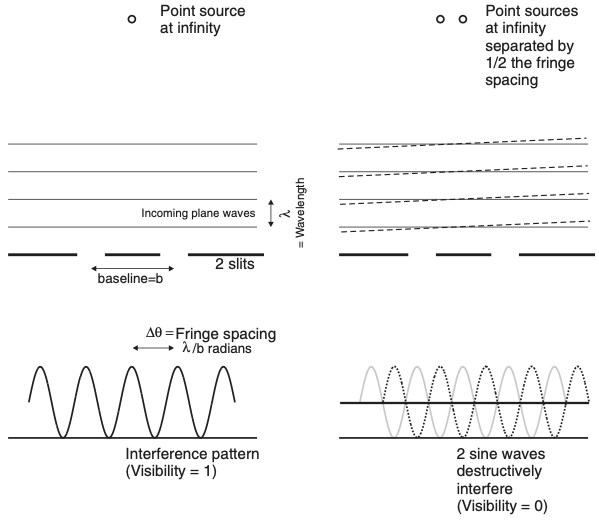
\includegraphics[width=0.8\textwidth]{doc/youngs.png}
    \caption{Illustration of Young's double slit experiment (\emph{left}), and the resulting intensity image when two point sources are observed (\emph{right}). Credit: \citet{2003RPPh...66..789M}.}
    \label{fig:youngs}
\end{figure}

To recap the double slit experiment, Figure \ref{fig:youngs} shows the expected fringe pattern for a point source at infinity and with slits that have a spacing $b$. In interferometry, this separation is commonly called a ``baseline''. We assume that we are using/observing light that has a limited range of wavelengths that is centered on $\lambda$. The fringe pattern then has a spacing of $\lambda/b$; this is the angle in radians between fringe peaks from the plane of the slits to the detector. The fringe pattern intensity $I$ is commonly written as
\begin{equation}\label{eq:fringepattern}
    I = 4 I_0 \cos^2 \frac{\delta}{2}
\end{equation}
where $I_0$ is the intensity that would have resulted from light passing through a single hole or slit, and where $\delta$ is the phase difference that results from the different path lengths from the slits to a given point on the detector.

Now consider a second source of equal brightness, with an angular separation from the first of $\lambda/(2b)$. The fringes produced by this source will be 180$^\circ$ out of phase compared to the fringes from the first source, so will cancel. Because we are considering an analogy with an astronomical observation, the two sources are expected to be incoherent because their spatial separation will typically be large (e.g. millions of km apart on the surface of a star) and there is no reason to believe there is any laser-like behaviour that synchronises photon phases, so the phases of two photons coming from the two sources will have random phases with respect to each other. Thus, at any point on the detector we can simply add the intensity from the two independent fringe patterns (there is no sustained interference between the two patterns). For the case with the second source separated by $\lambda/(2b)$, the result is therefore no fringes at all, as shown in the right panel of Figure \ref{fig:youngs}. This disappearance of the fringes is how we define the resolution of an interferometer, while for single-dish (normal) telescopes with diameter $D$ it is the Rayleigh criterion of 1.22\,$\lambda/D$, for interferometers it is $\lambda/(2b)$.

\begin{figure}[h]
    \centering
    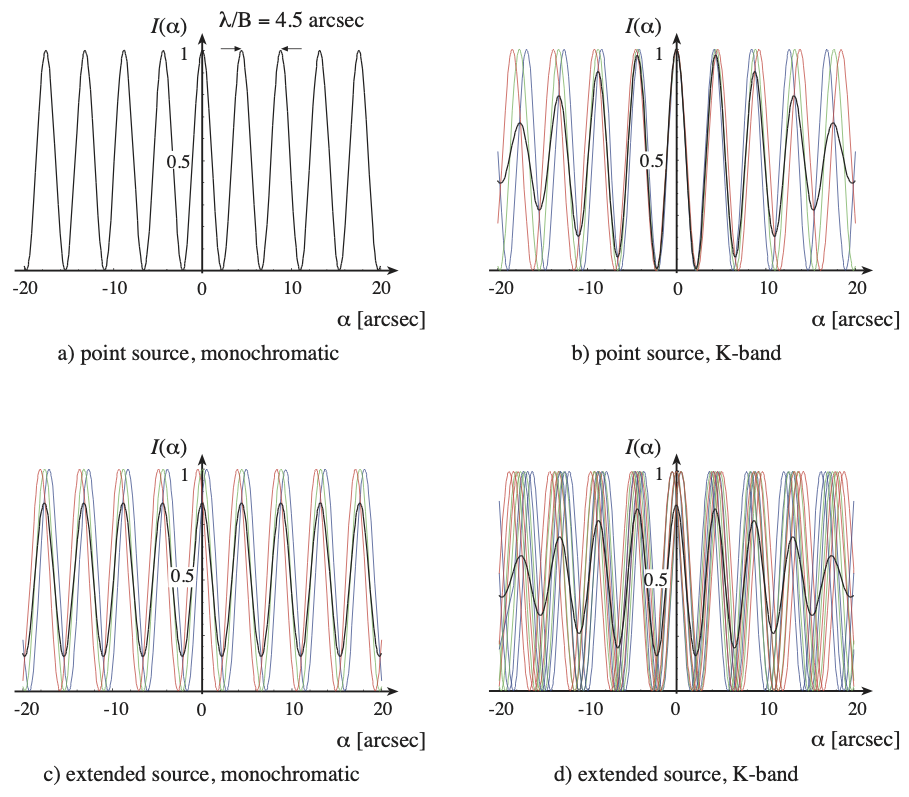
\includegraphics[width=0.8\textwidth]{doc/coherence.png}
    \caption{Illustration of how the fringe pattern is altered by a finite range of wavelengths and an extended source size (assuming a baseline of 10\,cm). Each panel shows several of the fringe patterns that are being superimposed, which result in the overall pattern shown as the thicker black line. The top left panel shows the fringe pattern for a monochromatic point source, and the other panels show how the fringe amplitude is reduced. The top right shows the effect for a range of wavelengths in the `K' band (near 2.5\,$\mu$m). The lower left panel shows the effect for an extended source, and the lower right panel the combination of an extended source and range of wavelengths. Credit: \href{https://www.eso.org/sci/facilities/paranal/telescopes/vlti/tuto/tutorial_spatial_interferometry.pdf}{Andreas Glindemann/ESO}}
    \label{fig:coherence}
\end{figure}

In intermediate cases where a second source is less separated, e.g. at $\lambda/(4b)$, the fringe patterns do not add up to a constant, but the amplitude of the pattern is still reduced. The same behaviour is typically observed when the source is extended, e.g. a uniform disk such as a stellar surface, since this case can be considered as the summation of a series of point sources. This reduction is illustrated in Figure \ref{fig:coherence}, most importantly in the lower left panel which considers a finite continuous source. A finite range of wavelengths will also reduce the fringe amplitude, though in this experiment we will ignore this effect.

In interferometry we are primarily interested in the amplitude of the fringes formed on our detector. We characterise this amplitude with the ``visibility'', which is defined as
\begin{equation}
    V = \frac{I_{\rm max} - I_{\rm min}}{I_{\rm max} + I_{\rm min}} \, .
\end{equation}
Looking at Figure \ref{fig:coherence}, we can see that the fringes in the top left panel have $V=1$ (and in the left panel of Figure \ref{fig:youngs}). For resolved sources the visibility is lower, for example in the lower left panel the value is about 0.6. For the right panel in Figure \ref{fig:youngs} the visibility is zero.

In general, the fringes are an indication of how well ``resolved'' a source is. An unresolved source will have strong fringes and a high visibility, but as the source becomes more extended the fringes weaken and the visibility drops. For continuous sources as we will be considering here, which are analogous to the surface of a star for example, when the source is larger than about $\lambda/(2b)$ the visibility drops to near zero. This can be understood as the image on the detector being the superposition of many fringes that have such a wide range of phases that the average is a constant.

Of course, in reality we do not change the source size, we instead change the resolution of our instrument, either by changing the wavelength $\lambda$ or the baseline length $b$. A typical measurement therefore normally consists of making visibility measurements for a range of wavelengths and baseline lengths, and using these to infer spatial information about our source.

Note that as we are only using a pair of baselines, we are really only measuring the source size along an axis parallel with the baseline vector. For sources that are not rotationally symmetric, we can address this by rotating our baselines to a different angle with respect to the source and making more measurements.

\subsection{Visibility functions}

Mathematically, we can write down the expected behaviour of the visibility as a function of baseline and wavelength for a few different source geometries. Some more detail on where these come from is \href{https://www.eso.org/sci/facilities/paranal/telescopes/vlti/tuto/tutorial_interferometry.html}{on this ESO page}.

The visibility for a binary source is perhaps not too surprising, we saw above that $V=1$ when their separation is zero, and $V=0$ when their separation is $\lambda/(2b)$, and $V$ varies sinusoidally in between. For a equal brightness binary with separation $s$, the visibility is
\begin{equation}
    V_{\rm binary} = \frac{1 + \cos ( 2 \pi s b / \lambda )}{2} \, .
\end{equation}

For an extended circular source of diameter $\theta$ as a function of baseline length the visibility is
\begin{equation}
    V_{\rm uniform} = \frac{2 J_1(\pi \theta b / \lambda)}{\pi \theta b / \lambda} \, ,
\end{equation}
where $J_1$ is a first order Bessel function.

These are the two main visibility functions that you will need for this experiment.

\section{Experimental setup}

This lab has an intentionally simple setup; the goal is to show how one can construct an interferometer from a standard telescope with minor and straightforward modifications. The key pieces of equipment are:
\begin{itemize}
    \item telescope, this is mounted to the bench
    \item CMOS detector and USB cable
    \item lens cap, this holds the tokens with the pairs of holes (baselines)
    \item baseline tokens, these have small (0.3\,mm) holes drilled in pairs with a range of separations
    \item light source
    \item aperture tokens, these go in front of the light source and are what we observe
    \item filters, used to change the wavelength of the source
\end{itemize}

Setting up the experiment is reasonably simple, the aim being to have the telescope pointed at the light source and aperture. While having the telescope properly focussed will aid the setup, it's not actually critical for observing the fringes. A suggested series of steps to get your first set up fringes is as follows:

\begin{enumerate}
    \item Plug the light source in to charge. The battery should last for hours, but it's best to turn it off when you're not using it.
    \item Ensure the telescope is in place with the lens cap on (no tokens needed yet).
    \item Insert the CMOS detector into the rear of the telescope and (gently) tighten the screws to keep it in place. You may end up rotating the detector later.
    \item Connect the CMOS detector to the computer with the USB cable.
    \item Open the image capture software (see \ref{sec:software}). The detector should be automatically recognised and an image appear on screen. Test whether the detector is working by covering/uncovering the hole in the lens cap.
    \item Set up the holder for the filters and aperture tokens. Place an aperture token in one of the slots.
    \item Remove the telescope lens cap and set up the focus and pointing. The telescope is fixed, so you will need to adjust the location of the filter/aperture holder until it appears near the center of the detector image. You will simultaneously need to adjust the focus so you know what you are pointing at. You may find it helpful to hold a large object (e.g. a book) in front of the holder to figure out where you need to point. You should end up with an in focus image of the aperture on the detector.
    \item Set up the light source behind the aperture, fixing it to the bench with clamps. Point it towards the telescope. The pointing doesn't need to be too precise; you can test whether it's pointing in the right direction by holding your hand in front of the aperture to see if the light is pointing towards the telescope.
    \item Insert one of the baseline tokens into the lens cap. You should now see fringes on the detector with an image similar to Figure \ref{fig:det-img}, though may need to alter the exposure time (around 1\,s should be enough).
\end{enumerate}

If all of this setup has gone well, you are now ready to start!

\subsection{Image capture software}\label{sec:software}

The software for this experiment is \href{http://www.firecapture.de/}{\texttt{firecapture}}; it is an open source code primarily designed for amateur astronomers, and provides a friendly and easy to use interface for viewing images from the detector in real time, and allows saving of images in various formats. A copy of the software should exist on the computer near where the telescope is set up. This is the computer you will plug the USB cable from the detector into.

\begin{figure}[h]
    \centering
    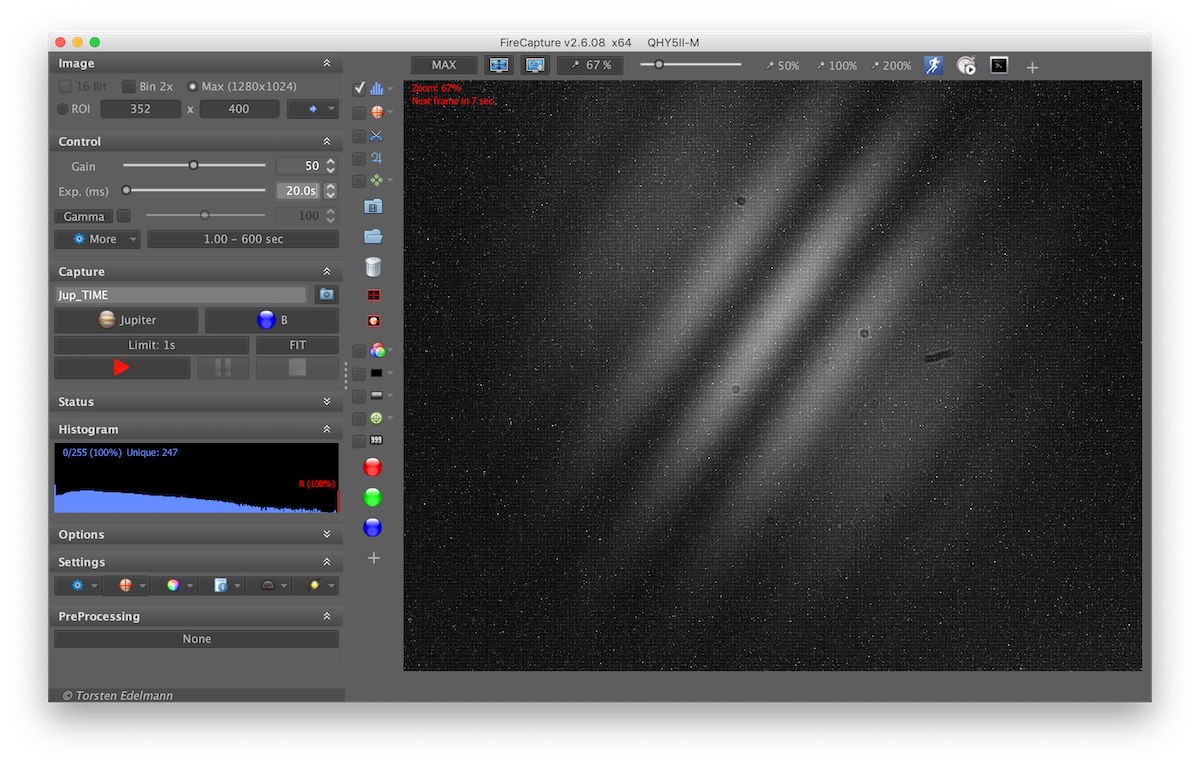
\includegraphics[width=1\textwidth]{doc/fc.png}
    \caption{Screenshot of the \texttt{firecapture} software running. The deteector image is in the main panel, and various controls are in the left column.}
    \label{fig:fc}
\end{figure}

You will not need most of the options available in \texttt{firecapture}. The main one in terms of obtaining images on screen is the exposure time (under ``control''); you will need to experiment, but values of about 1s are likely to be about right. The exposure time will however depend on what value you select for the gain. You will know the exposure is appropriate when you have an image visible on screen, and this image is not saturated (the ``histogram'' panel may help here).

The other important control is how images are saved (under ``capture''); for this you need to specify a directory in which to save images, a file format (select ``FIT''), and a number of images to save (just one, since you will hit save manually each time you change the baseline token, filter, etc.).

You can optionally save a ``dark frame'' (one of the small buttons between the main image and the left column of controls). This involves covering the front of the telescope (putting your hand in front of the baseline token would suffice) and taking an image that will be subtracted off subsequent images. The goal is that this dark image will contain any ``hot'' (permanently defective) detector pixels, and by subtracting them these pixels will not affect the final images.

\section{Measuring visibilities}\label{sec:meas}

The key measurement in this experiment is of the fringe visibility. In the images this is essentially how strong the fringes are; if their amplitude covers the full range from peak to the background level the visibility is high (i.e. near 1), and if they are barely visible then the visibility is low (i.e. near zero).

\begin{figure}[h]
    \centering
    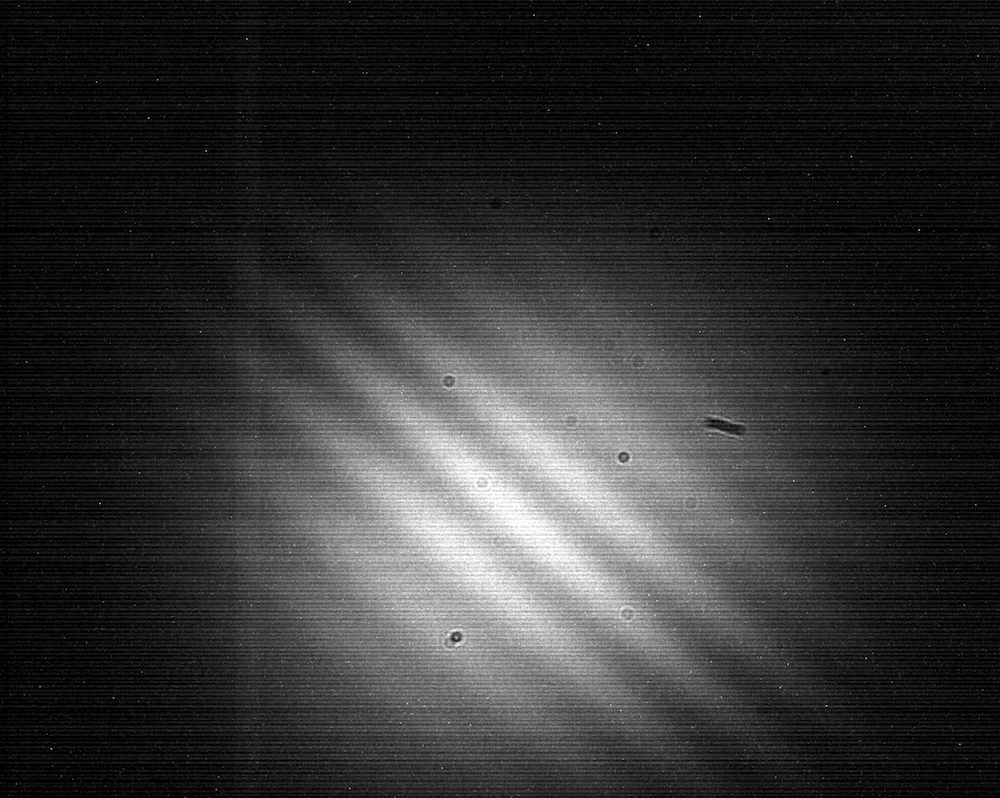
\includegraphics[width=0.8\textwidth]{doc/det-img.png}
    \caption{Example image. The broad circular envelope is the PSF, on which the fringes are superimposed. The small dots are aretefacts from dust somewhere in the optical path, likely on the detector.}
    \label{fig:det-img}
\end{figure}

There are three components that contribute to an image, an example is shown in Figure \ref{fig:det-img}:
\begin{itemize}
    \item background; this is contributed by any stray light that reaches the detector, plus any intrinsic level attributed to the detector itself
    \item point spread function (PSF); this is the broad overall shape of the signal on the detector and is approximately Gaussian, and is set by the size of the individual holes in the baseline tokens. Smaller holes yield a larger diffraction pattern, and vice versa.
    \item fringes; this is the fringe pattern resulting from the pair of holes
\end{itemize}
The goal in making a measurement is to subtract (or otherwise account for) the background, and make a measurement of the fringe visibility that (if possible/necessary) takes the shape of the PSF into account.

The simplest method for obtaining a visibility measurement would be to measure the background level somewhere away from the PSF, take peak and trough measurements for the fringes, subtract the background level from these, and then compute the visibility. A more complex, but more reliable method, is to use the supplied python widget (\texttt{widget.py}); this code models the above components of the detector image to come up with a parameterised fit to the data, from which the visibility can be extracted.

\subsection{Using \texttt{widget.py}}\label{sec:widget}

This code brings up an interactive window that allows a parameterised fit to a detector image, and which will output the model parameters, including the visibility and baseline angle (with respect to the detector, whose orientation depends on how you insert it into the telescope). The code itself exists on github\footnote{\href{https://github.com/drgmk/px-interferometry}{https://github.com/drgmk/px-interferometry}}, you can download it from here if it is not already on the machine you are using.

\section{The experiment}

There are many possible measurements that could be made with this experimental setup. The two key ones you should do are to i) measure the angular size of a source (i.e. aperture), and to ii) verify the expected visibility variation with baseline for a binary source. Beyond these two possible options are to iii) characterise the shape of a non-rotationally symmetric source, iv) try repeating one of parts i/ii, but using Fourier transforms to extract the visibilities from the data, v) create your own baseline token with more than 2 holes using tin foil and a pin, and use this to take some measurements (e.g. to measure an aperture size and/or shape).

\subsection{Basic procedure}

The basic procedure for this experiment is to set things up as you desire, verify the setup is working visually using the image on the screen, and to then save that image. These steps are then repeated as necessary to obtain a full set of images, e.g. across several baselines with different filters. The resulting images are then analysed to obtain visibility measurements, and these visibilities are then used in concert with the baseline length and filter wavelength information to obtain a result. This result would typically be a plot of baseline vs. $b/\lambda$, and/or a fit to the relevant theoretical curve to obtain an estimate of the source aperture size.

\bibliographystyle{aasjournal}
\bibliography{refs}

\end{document}  